%  A simple AAU report template.
%  2015-05-08 v. 1.2.0
%  Copyright 2010-2015 by Jesper Kjær Nielsen <jkn@es.aau.dk>
%
%  This is free software: you can redistribute it and/or modify
%  it under the terms of the GNU General Public License as published by
%  the Free Software Foundation, either version 3 of the License, or
%  (at your option) any later version.
%
%  This is distributed in the hope that it will be useful,
%  but WITHOUT ANY WARRANTY; without even the implied warranty of
%  MERCHANTABILITY or FITNESS FOR A PARTICULAR PURPOSE.  See the
%  GNU General Public License for more details.
%
%  You can find the GNU General Public License at <http://www.gnu.org/licenses/>.
%
\documentclass[11pt,a4paper,openright]{report}
%%%%%%%%%%%%%%%%%%%%%%%%%%%%%%%%%%%%%%%%%%%%%%%%
% Language, Encoding and Fonts
% http://en.wikibooks.org/wiki/LaTeX/Internationalization
%%%%%%%%%%%%%%%%%%%%%%%%%%%%%%%%%%%%%%%%%%%%%%%%
% Select encoding of your inputs. Depends on
% your operating system and its default input
% encoding. Typically, you should use
%   Linux  : utf8 (most modern Linux distributions)
%            latin1 
%   Windows: ansinew
%            latin1 (works in most cases)
%   Mac    : applemac
% Notice that you can manually change the input
% encoding of your files by selecting "save as"
% an select the desired input encoding. 
\usepackage[utf8]{inputenc}
% Make latex understand and use the typographic
% rules of the language used in the document.
\usepackage[english, danish]{babel}
% Use the palatino font
\usepackage[sc]{mathpazo}
\linespread{1.05}         % Palatino needs more leading (space between lines)
% Choose the font encoding
\usepackage[T1]{fontenc}
%%%%%%%%%%%%%%%%%%%%%%%%%%%%%%%%%%%%%%%%%%%%%%%%
% Graphics and Tables
% http://en.wikibooks.org/wiki/LaTeX/Importing_Graphics
% http://en.wikibooks.org/wiki/LaTeX/Tables
% http://en.wikibooks.org/wiki/LaTeX/Colors
%%%%%%%%%%%%%%%%%%%%%%%%%%%%%%%%%%%%%%%%%%%%%%%%
% load a colour package
\usepackage[dvipsnames]{xcolor}
\definecolor{aaublue}{RGB}{33,26,82}% dark blue
% The standard graphics inclusion package
\usepackage{graphicx}
% Set up how figure and table captions are displayed
\usepackage{float}
\usepackage{caption}
\captionsetup{%
  font=footnotesize,% set font size to footnotesize
  labelfont=bf % bold label (e.g., Figure 3.2) font
}
% Make the standard latex tables look so much better
\usepackage{array,booktabs}
% Enable the use of frames around, e.g., theorems
% The framed package is used in the example environment
\usepackage{framed}
\usepackage{wrapfig}
\usepackage{multirow}

%%%%%%%%%%%%%%%%%%%%%%%%%%%%%%%%%%%%%%%%%%%%%%%%
% Mathematics
% http://en.wikibooks.org/wiki/LaTeX/Mathematics
%%%%%%%%%%%%%%%%%%%%%%%%%%%%%%%%%%%%%%%%%%%%%%%%
% Defines new environments such as equation,
% align and split 
\usepackage{amsmath}
% Adds new math symbols
\usepackage{amssymb}
% Use theorems in your document
% The ntheorem package is also used for the example environment
% When using thmmarks, amsmath must be an option as well. Otherwise \eqref doesn't work anymore.
\usepackage[framed,amsmath,thmmarks]{ntheorem}

%%%%%%%%%%%%%%%%%%%%%%%%%%%%%%%%%%%%%%%%%%%%%%%%
% Page Layout
% http://en.wikibooks.org/wiki/LaTeX/Page_Layout
%%%%%%%%%%%%%%%%%%%%%%%%%%%%%%%%%%%%%%%%%%%%%%%%
% Change margins, papersize, etc of the document
\usepackage[
  inner=30mm,% left margin on an odd page
  outer=30mm,% right margin on an odd page
  ]{geometry}
% Modify how \chapter, \section, etc. look
% The titlesec package is very configureable
\usepackage{titlesec}
\titleformat{\chapter}[display]{\normalfont\huge\bfseries}{\ }{20pt}{\Huge}
\titleformat*{\section}{\normalfont\Large\bfseries}
\titleformat*{\subsection}{\normalfont\large\bfseries}
\titleformat*{\subsubsection}{\normalfont\normalsize\bfseries}
\titleformat*{\paragraph}{\normalfont\normalsize\bfseries}
\titleformat*{\subparagraph}{\normalfont\normalsize\bfseries}

% Clear empty pages between chapters
\let\origdoublepage\cleardoublepage
\newcommand{\clearemptydoublepage}{%
  \clearpage
  {\pagestyle{empty}\origdoublepage}%
}
\let\cleardoublepage\clearemptydoublepage

% Change the headers and footers
\usepackage{fancyhdr}
\pagestyle{fancy}
\fancyhf{} %delete everything
\renewcommand{\headrulewidth}{0pt} %remove the horizontal line in the header
\fancyhead[R]{\small\nouppercase\leftmark} %even page - chapter title
\fancyhead[LO]{\small\nouppercase\rightmark} %uneven page - section title
\fancyhead[RO]{\thepage} %page number on all pages
\setlength{\headheight}{13.59999pt}
% Do not stretch the content of a page. Instead,
% insert white space at the bottom of the page
\raggedbottom
% Enable arithmetics with length. Useful when
% typesetting the layout.
\usepackage{calc}

%Paragraph spacing
\setlength{\parindent}{0em}
\setlength{\parskip}{1em}

%%%%%%%%%%%%%%%%%%%%%%%%%%%%%%%%%%%%%%%%%%%%%%%%
% Misc
%%%%%%%%%%%%%%%%%%%%%%%%%%%%%%%%%%%%%%%%%%%%%%%%
% Add bibliography and index to the table of
% contents
\usepackage[nottoc]{tocbibind}
% Add the command \pageref{LastPage} which refers to the
% page number of the last page
\usepackage{lastpage}
% Add todo notes in the margin of the document
\usepackage[
%  disable, %turn off todonotes
  colorinlistoftodos, %enable a coloured square in the list of todos
  textwidth=\marginparwidth, %set the width of the todonotes
  textsize=scriptsize, %size of the text in the todonotes
  ]{todonotes}
% include pdf files
\usepackage[final]{pdfpages}
% code
\usepackage{color}
\usepackage{listings}
\usepackage{tcolorbox}
\usepackage{subfig}
% coding colors defined %
\definecolor{codegreen}{rgb}{0,0.6,0}
\definecolor{codegray}{rgb}{0.5,0.5,0.5}
\definecolor{codepurple}{rgb}{0.58,0,0.82}
\definecolor{backcolour}{rgb}{0.95,0.95,0.92}

 
\lstdefinestyle{JavaStyle}{
    backgroundcolor=\color{backcolour},   
    commentstyle=\color{codegreen},
    keywordstyle=\color{magenta},
    numberstyle=\tiny\color{codegray},
    stringstyle=\color{codepurple},
    basicstyle=\footnotesize,
    breakatwhitespace=false,         
    breaklines=true,                 
    captionpos=b,
    frame=single,
    keepspaces=true,                 
    numbers=left,                    
    numbersep=5pt,                  
    showspaces=false,                
    showstringspaces=false,
    showtabs=false,
    language=Java,
    tabsize=4,
    extendedchars=true,
    literate={æ}{{\ae}}1 {Æ}{{\AE}}1 {ø}{{\o}}1 {Ø}{{\O}}1 {å}{{\r a}}1 {Å}{{\r A}}1,
}

\lstdefinelanguage{JavaScript}{
%alsoletter=æøå,
keywords={metode, liste, Dec, udskriv, hvis, tilføj, returner, hent, længde, somHeltal, Hel, imens, indsæt, ordbog, tekst, størrelse, nøgler},
keywordstyle=\color{blue}\bfseries,
ndkeywords={start},
ndkeywordstyle=\color{darkgray}\bfseries,
identifierstyle=\color{black},
sensitive=false,
comment=[l]{//},
morecomment=[s]{/*}{*/},
commentstyle=\color{purple}\ttfamily,
stringstyle=\color{red}\ttfamily,
morestring=[b]',
morestring=[b]"
}

\lstdefinestyle{JavaScriptStyle}{
    backgroundcolor=\color{backcolour},   
    commentstyle=\color{codegreen},
    keywordstyle=\color{magenta},
    numberstyle=\tiny\color{codegray},
    stringstyle=\color{codepurple},
    basicstyle=\footnotesize,
    breakatwhitespace=false,         
    breaklines=true,                 
    captionpos=b,
    frame=single,
    keepspaces=true,                 
    numbers=left,                    
    numbersep=5pt,                  
    showspaces=false,                
    showstringspaces=false,
    showtabs=false,
    language=javascript,
    tabsize=4,
    extendedchars=true,
    literate={æ}{{\ae}}1 {Æ}{{\AE}}1 {ø}{{\o}}1 {Ø}{{\O}}1 {å}{{\r a}}1 {Å}{{\r A}}1,
}
\lstset{style=JavaStyle}
\renewcommand{\lstlistingname}{Code}% Listing -> Code
\renewcommand{\lstlistlistingname}{List of \lstlistingname}% List of Listings -> List of Code
%%%%%%%%%%%%%%%%%%%%%%%%%%%%%%%%%%%%%%%%%%%%%%%%
% Hyperlinks
% http://en.wikibooks.org/wiki/LaTeX/Hyperlinks
%%%%%%%%%%%%%%%%%%%%%%%%%%%%%%%%%%%%%%%%%%%%%%%%
% Enable hyperlinks and insert info into the pdf
% file. Hypperref should be loaded as one of the 
% last packages

\usepackage{multirow}
\usepackage{csquotes}
\usepackage{chngpage}
\usepackage{pdflscape}
\usepackage{longtable}
\usepackage{makecell}

\usepackage[nobreak]{mdframed}

\numberwithin{equation}{chapter}

\usepackage{csvsimple}

\usepackage{tikz}
\usetikzlibrary{matrix}

\titlespacing*{\chapter}{0pt}{0pt}{40pt}
\usepackage{ulem}

\mdfdefinestyle{drikstyle}{%
linecolor=CornflowerBlue,linewidth=2pt,%
frametitlerule=true,%
frametitlebackgroundcolor=CornflowerBlue!20,
innertopmargin=\topskip,
}
\mdtheorem[style=drikstyle]{drik}{Drik}

\mdfdefinestyle{særligstyle}{%
linecolor=SpringGreen,linewidth=2pt,%
frametitlerule=true,%
frametitlebackgroundcolor=SpringGreen!20,
innertopmargin=\topskip,
}
\mdtheorem[style=særligstyle]{særlig}{Særlig}

\mdfdefinestyle{giftstyle}{%
linecolor=Bittersweet,linewidth=2pt,%
frametitlerule=true,%
frametitlebackgroundcolor=Bittersweet!20,
innertopmargin=\topskip,
}
\mdtheorem[style=giftstyle]{gift}{Gift}

\mdfdefinestyle{artefaktstyle}{%
linecolor=BlueGreen,linewidth=2pt,%
frametitlerule=true,%
frametitlebackgroundcolor=BlueGreen!20,
innertopmargin=\topskip,
}
\mdtheorem[style=artefaktstyle]{artefakt}{Artefakt}

\mdfdefinestyle{runerustningstyle}{%
linecolor=Emerald,linewidth=2pt,%
frametitlerule=true,%
frametitlebackgroundcolor=Emerald!20,
innertopmargin=\topskip,
}
\mdtheorem[style=runerustningstyle]{runerustning}{Runerustning}

\mdfdefinestyle{runevåbenstyle}{%
linecolor=RoyalBlue,linewidth=2pt,%
frametitlerule=true,%
frametitlebackgroundcolor=RoyalBlue!20,
innertopmargin=\topskip,
}
\mdtheorem[style=runevåbenstyle]{runevåben}{Runevåben}

\mdfdefinestyle{runeskjoldstyle}{%
linecolor=RoyalPurple,linewidth=2pt,%
frametitlerule=true,%
frametitlebackgroundcolor=RoyalPurple!20,
innertopmargin=\topskip,
}
\mdtheorem[style=runeskjoldstyle]{runeskjold}{Runeskjold}

\usepackage{tablefootnote}

\mdfdefinestyle{Meditationstyle}{%
linecolor=Emerald,linewidth=2pt,%
frametitlerule=true,%
frametitlebackgroundcolor=Emerald!20,
innertopmargin=\topskip,
}
\mdtheorem[style=Meditationstyle]{meditation}{Meditation}

\mdfdefinestyle{Orleksarvstyle}{%
linecolor=RedOrange,linewidth=2pt,%
frametitlerule=true,%
frametitlebackgroundcolor=RedOrange!20,
innertopmargin=\topskip,
}
\mdtheorem[style=Orleksarvstyle]{orleks arv}{Orleks arv}
\mdtheorem[style=Orleksarvstyle]{dHævn}{Dæmonisk hævn}

\mdfdefinestyle{Ritualstyle}{%
linecolor=Magenta,linewidth=2pt,%
frametitlerule=true,%
frametitlebackgroundcolor=Magenta!20,
innertopmargin=\topskip,
}
\mdtheorem[style=Ritualstyle]{ritual}{Ritual}

\mdfdefinestyle{Åndensgavestyle}{%
linecolor=RoyalBlue,linewidth=2pt,%
frametitlerule=true,%
frametitlebackgroundcolor=RoyalBlue!20,
innertopmargin=\topskip,
}
\mdtheorem[style=Åndensgavestyle]{åndens gave}{Åndernes gave}

\mdtheorem[style=Meditationstyle]{nBeskyt}{Naturens Beskyttelse}

\mdfdefinestyle{naturstyle}{%
linecolor=Goldenrod,linewidth=2pt,%
frametitlerule=true,%
frametitlebackgroundcolor=Goldenrod!20,
innertopmargin=\topskip,
}
\mdtheorem[style=naturstyle]{nly}{Naturens Ly}

\mdtheorem[style=drikstyle]{nvit}{Naturens Vitalitet}

\mdtheorem[style=særligstyle]{mkær}{Moder Naturs Kærlighed}

\mdtheorem[style=giftstyle]{nhævn}{Naturens hævn}

\mdtheorem[style=Åndensgavestyle]{nkaos}{Naturens Kaos}

\mdtheorem[style=runeskjoldstyle]{nbesk}{Naturens Beskyttelse}

\mdfdefinestyle{primærstyle}{%
linecolor=Plum,linewidth=2pt,%
frametitlerule=true,%
frametitlebackgroundcolor=Plum!20,
innertopmargin=\topskip,
}
\mdtheorem[style=primærstyle]{primærMagi}{Primær Magi}

\mdfdefinestyle{Lærdstyle}{%
linecolor=SkyBlue,linewidth=2pt,%
frametitlerule=true,%
frametitlebackgroundcolor=SkyBlue!20,
innertopmargin=\topskip,
}
\mdtheorem[style=Lærdstyle]{lærdMagi}{Den Lærdes Vej}

\mdfdefinestyle{ArkBanestyle}{%
linecolor=SeaGreen,linewidth=2pt,%
frametitlerule=true,%
frametitlebackgroundcolor=SeaGreen!20,
innertopmargin=\topskip,
}
\mdtheorem[style=ArkBanestyle]{arkBaneMagi}{Arkanaens Bane}

\mdfdefinestyle{magiMesterstyle}{%
linecolor=Orange,linewidth=2pt,%
frametitlerule=true,%
frametitlebackgroundcolor=Orange!20,
innertopmargin=\topskip,
}
\mdtheorem[style=magiMesterstyle]{mesterMagi}{Magiens Mester}

\mdfdefinestyle{sAritstyle}{%
linecolor=Melon,linewidth=2pt,%
frametitlerule=true,%
frametitlebackgroundcolor=Melon!20,
innertopmargin=\topskip,
}
\mdtheorem[style=sAritstyle]{sAritMagi}{Sfære Aritmetik}

\usepackage[T1]{fontenc} %thanks's daleif
\usepackage[utf8]{inputenc}
\usepackage[english, danish]{babel}
\newcommand{\tabitem}{~~\llap{\textbullet}~~}

\mdfdefinestyle{racestyle}{%
linecolor=PineGreen,linewidth=2pt,%
frametitlerule=true,%
frametitlebackgroundcolor=PineGreen!20,
innertopmargin=\topskip,
}
\mdtheorem[style=sAritstyle]{race}{Race Detaljer}

\mdfdefinestyle{sjælstyle}{%
linecolor=Cyan,linewidth=2pt,%
frametitlerule=true,%
frametitlebackgroundcolor=Cyan!20,
innertopmargin=\topskip,
}
\mdtheorem[style=sjælstyle]{sjæl}{Sælg din Sjæl}

\mdfdefinestyle{Korruptionstyle}{%
linecolor=PineGreen,linewidth=2pt,%
frametitlerule=true,%
frametitlebackgroundcolor=PineGreen!20,
innertopmargin=\topskip,
}
\mdtheorem[style=Korruptionstyle]{korruption}{Korruption}

\mdfdefinestyle{Faldenstyle}{%
linecolor=Tan,linewidth=2pt,%
frametitlerule=true,%
frametitlebackgroundcolor=Tan!20,
innertopmargin=\topskip,
}
\mdtheorem[style=Faldenstyle]{falden}{Falden Engel}

\mdfdefinestyle{Vandstyle}{%
linecolor=Aquamarine,linewidth=2pt,%
frametitlerule=true,%
frametitlebackgroundcolor=Aquamarine!20,
innertopmargin=\topskip,
}
\mdtheorem[style=Vandstyle]{vand}{Vand}

\mdfdefinestyle{Ildstyle}{%
linecolor=BrickRed,linewidth=2pt,%
frametitlerule=true,%
frametitlebackgroundcolor=BrickRed!20,
innertopmargin=\topskip,
}
\mdtheorem[style=Ildstyle]{ild}{Ild}

\mdfdefinestyle{Jordstyle}{%
linecolor=Sepia,linewidth=2pt,%
frametitlerule=true,%
frametitlebackgroundcolor=Sepia!20,
innertopmargin=\topskip,
}
\mdtheorem[style=Jordstyle]{jord}{Jord}

\mdfdefinestyle{Vindstyle}{%
linecolor=Gray,linewidth=2pt,%
frametitlerule=true,%
frametitlebackgroundcolor=Gray!20,
innertopmargin=\topskip,
}
\mdtheorem[style=Vindstyle]{vind}{Vind}

\mdtheorem[style=naturstyle]{passiv}{Passiv}

\mdtheorem[style=ArkBanestyle]{offensiv}{Offensiv}

\mdtheorem[style=runevåbenstyle]{defensiv}{Defensiv}

\mdtheorem[style=giftstyle]{kontrol}{Kontrol}

\mdtheorem[style=særligstyle]{zombie}{Zombie}

\mdtheorem[style=Orleksarvstyle]{nSjæl}{Sjæl}

\mdtheorem[style=Åndensgavestyle]{sygdom}{Sygdomens Mørke}

\mdtheorem[style=Ritualstyle]{død}{Død}

\mdtheorem[style=Ritualstyle]{prof}{Profession}% package inclusion and set up of the document
% see, e.g., http://en.wikibooks.org/wiki/LaTeX/Formatting#Hyphenation
% for more information on word hyphenation
\hyphenation{ex-am-ple hy-phen-a-tion short}
\hyphenation{long la-tex}% 
%  A simple AAU report template.
%  2015-05-08 v. 1.2.0
%  Copyright 2010-2015 by Jesper Kjær Nielsen <jkn@es.aau.dk>
%
%  This is free software: you can redistribute it and/or modify
%  it under the terms of the GNU General Public License as published by
%  the Free Software Foundation, either version 3 of the License, or
%  (at your option) any later version.
%
%  This is distributed in the hope that it will be useful,
%  but WITHOUT ANY WARRANTY; without even the implied warranty of
%  MERCHANTABILITY or FITNESS FOR A PARTICULAR PURPOSE.  See the
%  GNU General Public License for more details.
%
%  You can find the GNU General Public License at <http://www.gnu.org/licenses/>.
%
%
%
% see, e.g., http://en.wikibooks.org/wiki/LaTeX/Customizing_LaTeX#New_commands
% for more information on how to create macros

%%%%%%%%%%%%%%%%%%%%%%%%%%%%%%%%%%%%%%%%%%%%%%%%
% Macros for the titlepage
%%%%%%%%%%%%%%%%%%%%%%%%%%%%%%%%%%%%%%%%%%%%%%%%
%Creates the aau titlepage
\newcommand{\aautitlepage}[3]{%
  {
    %set up various length
    \ifx\titlepageleftcolumnwidth\undefined
      \newlength{\titlepageleftcolumnwidth}
      \newlength{\titlepagerightcolumnwidth}
    \fi
    \setlength{\titlepageleftcolumnwidth}{0.5\textwidth-\tabcolsep}
    \setlength{\titlepagerightcolumnwidth}{\textwidth-2\tabcolsep-\titlepageleftcolumnwidth}
    %create title page
    \thispagestyle{empty}
    \noindent%
    \begin{tabular}{@{}ll@{}}
      \parbox{\titlepageleftcolumnwidth}{
        \iflanguage{danish}{%
          \includegraphics[width=\titlepageleftcolumnwidth]{figures/aau_logo_da}
        }{%
          \includegraphics[width=\titlepageleftcolumnwidth]{figures/aau_logo_en}
        }
      } &
      \parbox{\titlepagerightcolumnwidth}{\raggedleft\sf\small
        #2
      }\bigskip\\
       #1 &
      \parbox[t]{\titlepagerightcolumnwidth}{%
      \textbf{Abstract:}\bigskip\par
        \fbox{\parbox{\titlepagerightcolumnwidth-2\fboxsep-2\fboxrule}{%
          #3
        }}
      }\\
    \end{tabular}
    \vfill
    \iflanguage{danish}{%
      \noindent{\footnotesize\emph{Rapportens indhold er frit tilgængeligt, men offentliggørelse (med kildeangivelse) må kun ske efter aftale med forfatterne.}}
    }{%
      \noindent{\footnotesize\emph{The content of this report is freely available, but publication (with reference) may only be pursued due to agreement with the author.}}
    }
    \clearpage
  }
}

%Create english project info
\newcommand{\englishprojectinfo}[8]{%
  \parbox[t]{\titlepageleftcolumnwidth}{
    \textbf{Title:}\\ #1\bigskip\par
    \textbf{Theme:}\\ #2\bigskip\par
    \textbf{Project Period:}\\ #3\bigskip\par
    \textbf{Project Group:}\\ #4\bigskip\par
    \textbf{Participant(s):}\\ #5\bigskip\par
    \textbf{Supervisor(s):}\\ #6\bigskip\par
    \textbf{Page Numbers:} \pageref{LastPage}\bigskip\par
    \textbf{Date of Completion:}\\ #8
  }
}

%Create danish project info
\newcommand{\danishprojectinfo}[8]{%
  \parbox[t]{\titlepageleftcolumnwidth}{
    \textbf{Titel:}\\ #1\bigskip\par
    \textbf{Tema:}\\ #2\bigskip\par
    \textbf{Projektperiode:}\\ #3\bigskip\par
    \textbf{Projektgruppe:}\\ #4\bigskip\par
    \textbf{Deltager(e):}\\ #5\bigskip\par
    \textbf{Vejleder(e):}\\ #6\bigskip\par
    \textbf{Oplagstal:} #7\bigskip\par
    \textbf{Sidetal:} \pageref{LastPage}\bigskip\par
    \textbf{Afleveringsdato:}\\ #8
  }
}

%%%%%%%%%%%%%%%%%%%%%%%%%%%%%%%%%%%%%%%%%%%%%%%%
% An example environment
%%%%%%%%%%%%%%%%%%%%%%%%%%%%%%%%%%%%%%%%%%%%%%%%
\theoremheaderfont{\normalfont\bfseries}
\theorembodyfont{\normalfont}
\theoremstyle{break}
\def\theoremframecommand{{\color{gray!50}\vrule width 5pt \hspace{5pt}}}
\newshadedtheorem{exa}{Example}[chapter]
\newenvironment{example}[1]{%
		\begin{exa}[#1]
}{%
		\end{exa}
}% my new macros
\usepackage{xcolor,colortbl}
\definecolor{Gray}{gray}{0.85}
\newcolumntype{a}{>{\columncolor{Gray}}c}
\newcolumntype{b}{>{\columncolor{white}}c}
\definecolor{maroon}{cmyk}{0,0.87,0.68,0.32}
\definecolor{bleudefrance}{rgb}{0.19, 0.55, 0.91}
\definecolor{cerulean}{rgb}{0.0, 0.48, 0.65}
\usepackage{hyperref}
\hypersetup{%
	%pdfpagelabels=true,%
	plainpages=false,%
	pdfauthor={Akastin},%
	pdftitle={Alkymist Regelsæt},%
	pdfsubject={Regler},%
	bookmarksnumbered=true,%
	colorlinks=true,%
	citecolor=black,%
	filecolor=blue,%
	linkcolor=black,% you should probably change this to black before printing
	urlcolor=blue,%
	pdfstartview=FitH,%
	bookmarksopen=true
}
\usepackage{stmaryrd}

\begin{document}
\begin{titlepage}
    \begin{center}
        \includegraphics[width=0.95\textwidth]{setup/Pictures/A01.C01.01_Front_Billede.png}
        
        \vspace{0.5cm}
        \LARGE
        \textit{Regelsæt til}
        
        \vspace{4.5cm}
        \Huge
        \textbf{Alkymist}\\
        \vspace{4.5cm}
        \large
        \textit{Opdateret: \today}
\end{center}
\end{titlepage}

\pagestyle{plain} %enable headers and footers again
%mainmatter
\pagenumbering{arabic} %use arabic page numbering in the mainmatter
\renewcommand*\contentsname{Indholdsfortegnelse}
\tableofcontents

\chapter{Indledning}

Denne profession kræver \textbf{ikke} special ansøgning.\\
Som alkymist kan du bruge alle typer rustning, med undtagelse af tårnskjolde, og du kan bruge våben som kun kræver en hånd. Det er yderligere muligt at lærer benyttelsen af to-håndsvåben gennem generelle evner.\\
Du kan maksimalt få 4 RP fra rustning, uanset hvor meget rustning du har. Det vil sige at selv hvis du får at vide at du har 13 RP ved tjek ind, så har du kun 4.\\

For at spille alkymist \textbf{skal} du selv medbringe følgende ting: Flasker til drikke, passende frugtfarve, og noget at brygge drikken i. Derudover er denne profession tiltænkt ældre spillere.\\

Alkymisten er en person der mestre evnen til at blande urter og andre sære ingredienser til diverse vidunderdrikke. Effekten af disse drikke er meget forskellig, hvilket også bevirker, at alkymister kan være meget forskellige. Det kan være alt fra en gal forsker, til en druide der lever i harmoni med naturen.
Som alkymist er det vigtigt at bære en masse tasker til opbevaring af de mange glas og urter det kræver at lave disse brygge. Dertil kan der tilføjes f.eks. en morter, som kan bruges til at knuse urter og planter, for at skabe disse mystiske drikke.\\
Det er vigtigt at fremhæve, at de drikke en alkymist producere ikke er magiske men kemiske. Det skal ligeledes understreges, at én flaske maks. kan indeholde én drik, samt at en person kun kan være påvirket af én positiv og én negativ drik af gangen.\\
\chapter{Drikke}

Med evnen Alkymi kan du lave drikke, der påvirker spillet og spillerne. De drikke, du kan lave med denne evne er ikke magiske, men kemiske.\\
Du kan blive påvirket af flere drikke på samme tid, men du kan ikke få den samme effekt fra den samme drik flere gange.\\
Drikke virker på 2 måder:
\begin{itemize}
    \item \textbf{Øjeblikkelig:} Disse drikke virker med de samme og effekten virker kun i det øjeblik de drikkes.
    \item \textbf{Over tid:} Disse drikke træder i kraft fra øjeblikket de indtages, og varer derefter over den tid, der beskrives på drikken.
\end{itemize}

Alle drikke holder indtil de er brugt, med få undtagelser. En drik kan derfor gemmes mellem spilgange, men vær dog opmærksom på at det er alkymistens ansvar, at indholdet ikke bliver for gammelt.\\
\textbf{\underline{Indholdet skal skiftes til hver scenarie!!}}

\section{Hvordan man brygger}
Af hensyn til spillet skal du selv anskaffe glas, flasker og diverse redskaber, som er passende til den type alkymist du spiller. En alkymist uden redskaber kan ikke brygge nogle drikke.\\
Rollespilsforeningen A’kastin kan \textbf{ikke} udlåne glas/flasker/diverse der kan benyttes til alkymi.\\
Flaskerne må ikke være for store, da indholdet skal kunne drikkes i en mundfuld.\\
For at skabe så meget spil som muligt, skal du huske at din rolle skal fremstå ægte, og give andre spillere mulighed for at reagere på dit arbejde. Derfor er det vigtigt at tage sig tid til brygningen. Det er ligeledes vigtigt, at du har alle ingredienserne der kræves til den specifikke drik.\\
\\\\\\
Når du har lavet din bryg, kan denne hældes på en flaske, hvorefter du kan sælge den. Den færdige drik skal kunne indtages og må derfor på ingen måde være sundhedsskadelig. Så selvom jord, bark, bær og andet fra skoven kan bruges til effekter i spillet, må drikken \textbf{ikke} indeholde dette. Drikken skal derfor indeholde en væske, såsom vand (gerne med frugtfarve eller saft), juice el. lign.\\
Det er alkymistens ansvar at sikre sig, at folk der indager drikken ikke er allergisk overfor ingredienserne i drikkene! Det er muligt at nogen er allergiske overfor nødder, mælk el. lign.\\
Hver drik der laves skal markeres med en seddel. Denne seddel skal påskrives drikkens navn, niveau og effekt. Effekten skal skrives på bagsiden, så det ikke er muligt for andre at læse drikkens effekt inden den indtages.\\

\emph{Eksempel: Forside: “Mortimors drik”. Bagside: “Dødens Essens. Du går på 0 LP”.}

\chapter{Opskrifter}
Alle opskrifter findes i dette regelsæt for din profession. Du skal kopiere opskrifterne over på et stykke in-game papir, som du kan have med i spillet. (In-game papir kan laves ved at dyppe almindeligt printerpapir i kaffe eller en stærk te for at give det farve)\\
Det er ikke tilladt at brygge efter hukommelsen.\\ Som Alkymist har du kendskab til alle drikke og gifte lige så snart du har Alkymi evnen der giver adgang til dem.\\
\begin{table}[H]
    \centering
    \begin{tabular}{|c|c|}
    \hline
    \rowcolor{cerulean!80}
        Niveau opskrift & Brygge tid \\\hline
        1 & 2 Minutter\\\hline
        2 & 4 Minutter \\\hline
        3 & 6 Minutter \\\hline
        4 & 8 Minutter \\\hline
    \end{tabular}
    \caption{Bryg tid}
    \label{tab:my_label}
\end{table}

\chapter{Ingredienser}
Hver opskrift kræver ingredienser. Ingredienserne i A'kastin vil altid bestå af en pose, der er markeret med ingrediensens navn. Når du har brugt en ingrediens afleveres den til en arrangør.\\
Der findes også ingredienser, som ikke gives ud af arrangørerne. Det kan for eksempel være øl fra kroen eller blod fra et offer. Uanset om ingrediensen er en væske eller et fast stof (for eksempel mos fra skoven), skal du bruge en beholder til at have ingrediensen i - meget gerne en beholder af glas. Vi gør opmærksom på, at alle drikke skal være drikkelige. Det vil sige ingen mos eller blade i dem.
\begin{center}
\begin{longtable}{|p{0.1\textwidth}|p{0.15\textwidth}|p{0.3\textwidth}|p{0.25\textwidth}|p{0.1\textwidth}|}
\hline
\rowcolor{cerulean!80}
Niveau & Navn & Beskrivelse & Effekt & Type \\\hline
\endhead

\hline \hline
\endlastfoot

1 & Blodbær &  Blodrøde bær. Dværgene kalder disse bær for Rustbær, da de ikke bliver lige så røde i Livet's ende. & Folk der spiser dem genvinder hurtigere kampkraft & Nyttig plante\\\hline
        
1 & Kongetand & En almindelig rod som mange koger suppe på. Normade stammer på De uendelige sletter bruger dem til at finde vand. & Denne rod hjælper med helbredelse. & Nyttig plante\\\hline

1 & Vorterod & En rod som findes under bøg træer. Den ligner en finger fyldt med vorter. & Folk der spiser den vil have mavepine. & Giftig plante \\\hline

2 & Ildgræs & Dette orange græs beklæder det meste af De Uendelige Sletter. & Dette græs kan antennes selvom det er vådt. & Nyttig plante \\\hline

2 & Kvælertang & Denne tang er kendt for at snøre sig omkring folk for at fortære deres krop under vandet. & Denne plante får blodet til at løbe langsommere & Giftig plante \\\hline

2 & Tudsebark & Denne bark samles fra sump træer i Mek og ligner en tudse set fra oven. & Denne bark fortynder blodet. & Giftig plante \\\hline

3 & Dværgerod & Denne plante menes at være i familie med Knoldselleri, denne art har dog et pragtfuld 'skæg' lavet af rødder. & Denne rod fortætter cellestrukturen. & Nyttig plante \\\hline

3 & Hybenholdt & Små spir fra en plante der normalt vokser omkring andre træer. & Denne plante er en kendt katalysator. & Nyttig plante \\\hline

3 & Slangefrø & Små frø fra en prægtig blomst. Når de rystes lyder de som en slange der hvæser. & Hvis disse frø spises skaber de illusioner. & Giftig plante \\\hline

4 & Cedertræ & Spåner fra et træ, som har været en stængel fra livets træ. & Te'en fra disse spåner har kraftige magiske og helbredende egenskaber. & Nyttig plante\\\hline

4 & Sort flue-svamp & En art af fluesvamp, som opstår når Ilsher blod rammer jorden. & Der findes ingen kendte arter som kan overleve at spise denne plante. & Giftig plante.\\\hline

\end{longtable}
\end{center}

\chapter*{Niveau 1}
\addcontentsline{toc}{chapter}{Niveau 1}
Du har lært at brygge lette drikke. Mange urter viser tydeligt deres potentiale, og du kan hjælpe dine venner i kamp.
\begin{table}[H]
    \centering
    \begin{tabular}{|p{0.50\textwidth}|p{0.25\textwidth}|}
    \rowcolor{cerulean!80}\hline
        Evne navn & Pris i XP \\\hline
         Alkymi Niv. 1 & 1 \\\hline
         Indkomst & 1 \\\hline
         Kemisk våben & 2 \\\hline
         Læse/Skrive Elvisk & 1\\
         \hline
    \end{tabular}
\end{table}

\section*{Evne beskrivelse}
\addcontentsline{toc}{section}{Evne beskrivelse}

\subsection*{Alkymi Niv. 1}
\addcontentsline{toc}{subsection}{Alkymi Niv. 1}
Du kan nu brygge en af de nedenstående drikke. Alle disse drikke kræver specifikke ingredienser, og kun du kan blande dem korrekt.\\

\begin{table}[H]
    \centering
    \begin{tabular}{|c|c|}
        \rowcolor{cerulean!80}\hline
        Drik & Gift \\\hline
        Enkens tåre &  Dværge snaps \\\hline
        Naturens bryg & Nervegift \\\hline
        Sten næver &  \\\hline
    \end{tabular}
    \caption{Oversigt over niveau 1 drikke.}
\end{table}

\begin{gift*}[Dværge snaps]
\textbf{Type:} Negativ Gift\\
\textbf{Ingredienser:} Øl fra kroen \& Vorterod\\
\textbf{Indtagelse:} Drikkes\\
\textbf{Effekt:} Ved indtagelse bliver man øjeblikkeligt meget beruset. Virkningen forsvinder, hvis spilleren mister bevidstheden eller 15 min efter indtagelse. Drikke efterlader ingen tømmermænd.\\
\end{gift*}

\begin{drik*}[Enkens tåre]
\textbf{Type:} Øjeblikkelig Drik\\
\textbf{Ingredienser:} Kongetand \& rent vand\\
\textbf{Indtagelse:} Drikkes\\
\textbf{Effekt:} Denne drik fjerne alle effekter af alkohol og gør øjeblikkeligt spilleren ædru. Dette betyder at de ikke vil være påvirket af alkohollet eller evner der kræver man er under effekten for alkohol.\\
\end{drik*}

\begin{drik*}[Naturens bryg]
    \textbf{Type:} Øjeblikkelig Drik\\
    \textbf{Ingredienser:} Ingen\\
    \textbf{Indtagelse:} Drikkes\\
    \textbf{Effekt:} Denne drik helbreder 1 LP. Du kan aldrig blive helbredt for mere end dit max LP.\\
    \textbf{Særligt:} Denne drik kan brygges hver anden time, men vare kun til slutningen af scenariet.
\end{drik*}

\begin{gift*}[Nervegift]
    \textbf{Type:} Øjeblikkelig Gift\\
    \textbf{Ingredienser:} Ingen\\
    \textbf{Indtagelse:} Drikkes / Blandes med væske\\
    \textbf{Effekt:}Denne drik skader 1 LP, og kan blandes i andre drikke uden, at den mister sin virkning.\\
   \textbf{Særligt:} Denne drik kan brygges hver anden time, men vare kun til slutningen af scenariet.
\end{gift*}

\begin{drik*}[Sten næver]
\textbf{Type:} Positiv drik\\
\textbf{Ingredienser:} 1 Dværgerod.\\
\textbf{Indtagelse:} Drikkes\\
\textbf{Effekt:} Når du drikker denne drik, får du +2NK i 30 min.
\end{drik*}


\subsection*{Indkomst}
\addcontentsline{toc}{subsection}{Indkomst}
Rul en 6-sidet terning ved tjek-in og få den mængde i Fjend\footnote{Møntfoden i A'kastin.} udleveret.

\subsection*{Kemisk våben}
\addcontentsline{toc}{subsection}{Kemisk våben}
Du kan nu påføre en gift på dit eget Våben. Det skal være et våben med klinge dvs. kniv, sværd eller lignende. Når du slår en person med dette våben vil ofret blive ramt af alle effekter som din gift har. Du kan kun ramme ét offer med giften, før en ny skal påføres. Du kan ikke give dit gift våben til andre. Vær opmærksom på at hvis du har den generelle evne, 'Påfør gift' vil du få XP prisen tilbage fra den evne når du køber Kemisk våben.\\

\subsection*{Læse/Skrive Elvisk}
\addcontentsline{toc}{subsection}{Læse/Skrive Elvisk}
Du kan læse og skrive skrift, der er skrevet på Elvisk.\\
\begin{figure}[H]
    \centering
    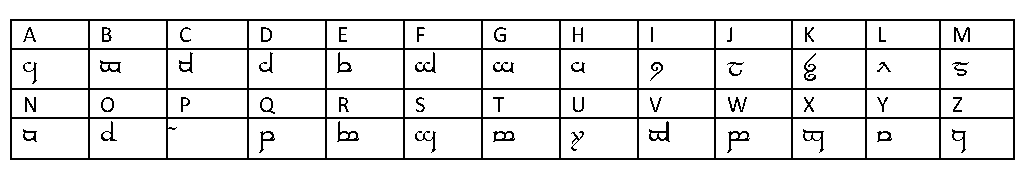
\includegraphics[width=1\textwidth]{setup/Alfabeter/Elvisk alfabet.pdf}
    \caption{Elvisk alfabet}
\end{figure}


\chapter{Niveau 2}
Du har lært at brygge de lidt mere avancerede drikke. Du kan se flere muligheder i mange af de urter du kender, og det er nu muligt for dig at påvirke spillet mere end før.\\
\begin{table}[H]
    \centering
    \begin{tabular}{|p{0.50\textwidth}|p{0.25\textwidth}|}
    \rowcolor{cerulean!80}\hline
        Evne navn & Pris i XP \\\hline
         Alkymi Niv. 2 & 2 \\\hline
         Bryggerens Hemmelighed Niv 1 & 2 \\\hline
         Læse/Skrive Magi & 1 \\\hline
         Personlig Have Niv. 1 & 2 \\
         \hline
    \end{tabular}
\end{table}
\section{Evne beskrivelse}

\subsection*{Alkymi Niv. 2}
\addcontentsline{toc}{subsection}{Alkymi Niv. 2}
Du kan nu brygge en af de nedenstående drikke ud over de drikke du har adgang til i niveau 1. Alle disse drikke kræver specifikke ingredienser, og kun du kan blande dem korrekt.\\

\begin{table}[H]
    \centering
    \begin{tabular}{|c|c|}
        \rowcolor{cerulean!80}\hline
        Drik & Gift \\\hline
        Blodorkens styrke &  Den lærtes mund \\\hline
        Drømmeløs hvile & Ewens humør \\\hline
        Helbredelsesdrik & Smertedrik \\\hline
        Kranieforstærker & Svag Giftdrik\\\hline
        Stenhud &  Søvndrik\\\hline
        \multicolumn{2}{|c|}{Speciel} \\\hline
        \multicolumn{2}{|c|}{Velsignet Olie} \\\hline
    \end{tabular}
    \caption{Oversigt over niveau 2 drikke.}
\end{table}

\begin{drik*}[Blodorkens styrke]
\textbf{Type:} Positiv drik \\
\textbf{Ingredienser:} 1 Dværgerod \& blod fra en blodork.\\
\textbf{Indtagelse:} Drikkes\\
\textbf{Effekt:} Når du drikker denne drik, får du +4NK i 30 min.
\end{drik*}

\begin{gift*}[Den lærtes mund]
\textbf{Type:} Negativ drik\\
\textbf{Ingredienser:} 3 Ildgræs\\
\textbf{Indtagelse:} Drikkes / Blandes med væske / Evnen Påfør Gift\\
\textbf{Effekt:} Den som indtager denne gift skal sige alt hvad de tænker, i de næste 10 minutter.
\end{gift*}

\begin{drik*}[Drømmeløs hvile]
\textbf{Type:} Positiv Drik\\
\textbf{Ingredienser:} Blodbær \& Kongetand \& Tudsebark \\
\textbf{Indtagelse:} Drikkes\\
\textbf{Effekt:} Når denne drik indtages, falder spilleren i søvn i 10 min. Efter disse 10 min vil alle naturlige LP være genvundet, men vækkes spilleren inden 10 min er gået, vil drikken ikke have nogen effekt og spilleren genvinder ingen LP.\\
\end{drik*}

\begin{gift*}[Ewens humør]
\textbf{Type:} Negativ drik\\
\textbf{Ingredienser:} Tudsebark \& Ildgræs\\
\textbf{Indtagelse:} Drikkes / Blandes med væske\\
\textbf{Effekt:} Når du drikker denne drik, er du venner med alt og alle og har bare lyst til at snakke med alle. Denne drik vare i 30 minutters.
\end{gift*}

\begin{drik*}[Helbredelsesdrik]
\textbf{Type:} Øjeblikkelig Drik\\
\textbf{Ingredienser:} 2 Kongetand\\
\textbf{Indtagelse:} Drikkes\\
\textbf{Effekt:} Denne drik helbreder 2 LP. Du kan aldrig blive helbredt for mere end dit max LP.\\
\end{drik*}


\begin{drik*}[Kranieforstærker]
\textbf{Type:} Positiv Drik\\
\textbf{Ingredienser:} Ildgræs \& Jern\\
\textbf{Indtagelse:} Drikkes\\
\textbf{Effekt:} Når du drikker denne drik bliver du immun overfor evnen Bonk de næste 30 min.\\
\end{drik*}

\begin{drik*}[Præstindens tårer]
\textbf{Type:} Øjeblikkelig Drik\\
\textbf{Ingredienser:} Velsignet vand \& Ildgræs \& Tudsebark \& Kongetand.\\
\textbf{Indtagelse:} Drikkes\\
\textbf{Effekt:} Fjerner alle positive og negative effekter fra Drikke og Gifte.
\end{drik*}

\begin{gift*}[Smertedrik]
\textbf{Type:} Negativ Gift\\
\textbf{Ingredienser:} 2 Vorterod\\
\textbf{Indtagelse:} Drikkes / Blandes med væske / Evnen Påfør Gift\\
\textbf{Effekt:} Den som indtager denne drik vil blive påvirket af smerte. Hvilket er en effekt, hvor du bliver ramt af en ulidelig smerte. Du skal derfor skrige og spille på, at du har ubærlige smerter i 30 sekunder.\\
\end{gift*}

\begin{drik*}[Stenhud]
\textbf{Type:} Positiv Drik\\
\textbf{Ingredienser:} Blod \& Kvælertang\\
\textbf{Indtagelse:} Drikkes\\
\textbf{Effekt:} Denne drik giver dig 2 LP over dit maks LP, som ikke kan genvindes. Effekten aftager, når der er gået 30 min eller, når du har mistet de ekstra LP.\\
\end{drik*}


\begin{gift*}[Svag Giftdrik]
\textbf{Type:} Øjeblikkelig Gift\\
\textbf{Ingredienser:} Tudsebark \& Vorterod\\
\textbf{Indtagelse:} Drikkes / Blandes med væske / Evnen Påfør Gift\\
\textbf{Effekt:} Når du bliver forgiftet af denne drik, mister du 2 LP.\\
\end{gift*}

\begin{gift*}[Søvndrik]
\textbf{Type:} Negativ Gift\\
\textbf{Ingredienser:} 2 Kvælertang\\
\textbf{Indtagelse:} Drikkes / Blandes med væske / Evnen Påfør gift.\\
\textbf{Effekt:} Når du indtager denne drik, vil du falde i søvn og sove de næste 5 min.\\
\end{gift*}

\begin{særlig*}
\textbf{Type:} Særlig\\
\textbf{Ingredienser:} Velsignet vand, en helbredende drik, Blodbær.\\
\textbf{Indtagelse:} Smøres på en klinge.\\
\textbf{Effekt:} Klingen denne olie smøres på vil give helligskade de næste 30 minutter. Dette skal markeres med et grønt bånd.
\end{særlig*}

\subsection{Bryggerens Hemmelighed Niv 1}
Du er bedre til at udnytte urternes potentiale, og får nu 2 drikke hver gang du brygger én drik. Du får også 2 Gifte når du brygger en gift.\\
Denne evner virker for alle niveau 1 og 2 drikke/gifte.\\

\input{../Evne-Ordbog/Læse og skrive/Læse og skrive Magisk.tex}

\subsection{Personlig Have Niv. 1}
Som en del af din spilgang kan du vælge et område som skal være din have. Vi foreslår at dette område er afmærket så det er tydeligt.\\
I løbet af en spilgang kan du vælge at plante en urt i din have. Dette betyder at du mister en urt, men ved starten af næste spilgang vil du få 3 af denne urt tilbage.\\
Vi vil meget gerne opfordre spillere til at søge hjælp fra andre til at 'velsigne', 'luge' eller 'gøde' deres have så dette kan give godt spil.\\
\\

\chapter{Niveau 3}
Du har brygget nok gifte til at dræbe en hel flok får, og nok helbredelsesdrikke til at kunne brygge dem i søvne, og denne erfaring har gjort det muligt for dig at brygge stærkere drikke end du havde regnet med, da du blandende dem.

\begin{table}[H]
    \centering
    \begin{tabular}{|p{0.50\textwidth}|p{0.25\textwidth}|}
    \rowcolor{cerulean!80}\hline
        Evne navn & Pris i XP \\\hline
        Alkymi Niv. 3 & 2\\\hline
        Bryggerens Hemmelighed Niv. 2 & 2\\\hline
        Urte ekspert & 1\\\hline
        Personlig Have Niv. 2 & 2\\
         \hline
    \end{tabular}
\end{table}
\section{Evne beskrivelse}

\subsection*{Alkymi Niv. 3}
\addcontentsline{toc}{subsection}{Alkymi Niv. 3}
Du kan nu brygge en af de nedenstående drikke ud over de drikke du har adgang til i niveau 1 \& 2. Alle disse drikke kræver specifikke ingredienser, og kun du kan blande dem korrekt.\\

\begin{table}[H]
    \centering
    \begin{tabular}{|c|c|}
        \rowcolor{cerulean!80}\hline
        Drik & Gift \\\hline
        Enorm helbredelsesdrik & Giftdrik \\\hline
        Huskedrik &  Kærlighedsdrik \\\hline
        Jevans kur &  Paralysedrik \\\hline
        Stor Helbredelsesdrik & Raffeals hån  \\\hline
         & Sandhedsdrik  \\\hline
    \end{tabular}
    \caption{Oversigt over niveau 3 drikke.}
\end{table}

\begin{drik*}[Enorm helbredelsesdrik]
\textbf{Type:} Øjeblikkelig Drik\\
\textbf{Ingredienser:} 2 Dværgerod, 3 kongetand.\\
\textbf{Indtagelse:} Drikkes.
\textbf{Effekt:} Når du drikker denne drik, genvinder du 6LP. Du kan aldrig blive helbredt for mere end dit max. LP
\end{drik*}

\begin{gift*}[Giftdrik]
\textbf{Type:} Øjeblikkelig Gift \\
\textbf{Ingredienser:} Vorterod \& Tudsebark \& Kvælertang\\
\textbf{Indtagelse:} Drikkes / Blandes med væske / Evnen Påfør Gift\\
\textbf{Effekt:} Når du bliver forgiftet af denne drik mister du 3 LP.\\
\end{gift*}

\begin{drik*}[Huskedrik]
\textbf{Type:} Positiv drik\\
\textbf{Ingredienser:} 2 Ildgræs \& Hybenholt\\
\textbf{Indtagelse:} Drikkes\\
\textbf{Effekt:} Når du drikker denne drik, kan du huske alt hvad der er sket for 30 minutter siden. Den ophæver derfor glemsels effekter som magi eller dødsreglen\\
\end{drik*}

\begin{drik*}[Jevans kur]
\textbf{Type:} Positiv Drik\\
\textbf{Ingredienser:} Hybenholt \& Kvælertang \& Dværgerod\\
\textbf{Indtagelse:} Drikkes\\
\textbf{Effekt:} Denne drik får et offer til at sove i 5 min. Når personen vågner, vil han være helbredt for alle sygdomme. Bliver han vækket før de 5min vil sygdommen ikke blive kureret.\\
\end{drik*}

\begin{gift*}[Kærlighedsdrik]
\textbf{Type:} Negativ Gift\\
\textbf{Ingredienser:} Hybenholt \& Slangefrø\\
\textbf{Indtagelse:} Drikkes / Blandes med væske\\
\textbf{Effekt:} Den som indtager denne drik vil blive stærkt forelsket i den næste person han/hun ser. Effekten varer i 30 min efter du først får øje på en person af modsatte køn.\\
\end{gift*}

\begin{gift*}[Paralysedrik]
\textbf{Type:} Negativ Gift\\
\textbf{Ingredienser:} 2 Slangefrø \& Vorterod \& Kvælertang\\
\textbf{Indtagelse:} Drikkes / Blandes med væske / Evnen Påfør Gift\\
\textbf{Effekt:} Den som indtager denne drik vil blive paralyseret i 30 sek.\\
\end{gift*}

\begin{gift*}[Raffeals hån]
\textbf{Type:} Negativ drik\\
\textbf{Ingredienser:} Slangefrø \& Tudsebark \& Kvælertang\\
\textbf{Indtagelse:} Drikkes / Blandes med væske / Evnen Påfør Gift\\
\textbf{Effekt:} Den som indtager denne drik vil ikke kunne tale sandt i de næste 30 min.\\
\textbf{Vigtigt:} Hvis du ville være tvunget til at tale sandt, fx gennem tortur, vil du ikke kune sige noget.
\end{gift*}

\begin{gift*}[Raffeals Vrede]
\textbf{Type:} Negativ Gift\\
\textbf{Ingredienser:} 1 Slangefrø \& 1 Hybenholt \\
\textbf{Indtagelse:} Drikkes / Blandes med væske\\
\textbf{Effekt:} Når du drikker denne drik, Hader du den første person du ser ubeskriveligt meget. Denne drik vare i 30 minutters.
\end{gift*}

\begin{gift*}[Sandhedsdrik]
\textbf{Type:} Negativ Gift\\
\textbf{Ingredienser:} Blodbær \& Hybenholt \& Slangefrø\\
\textbf{Indtagelse:} Drikkes / Blandes med væske / Evnen Påfør Gift\\
\textbf{Effekt:} Den som indtager denne drik kan KUN tale sandt og vil altid svare på spørgsmål uanset hvem, der spørger, så længe de er under drikkens effekt. Effekten virker i 10 min \\
\end{gift*}

\begin{drik*}[Stor Helbredelsesdrik]
\textbf{Type:} Øjeblikkelig Drik\\
\textbf{Ingredienser:} Dværgerod \& 2 Kongetand\\
\textbf{Indtagelse:} Drikkes\\
\textbf{Effekt:} Når du drikker denne drik genvinder du 4LP. Du kan aldrig blive helbredt for mere end dit max. LP\\
\end{drik*}


\subsection{Bryggerens Hemmelighed Niv 2}
Du er bedre til at udnytte urternes potentiale, og får nu 2 drikke hver gang du brygger én drik. Du får også 2 Gifte når du brygger en gift.\\
Denne evner virker for alle niveau 3 drikke/gifte.\\

\subsection{Urte ekspert}
Du kan tage med en person som bruger handelspoint. Når de Ekspresskøber Urter vil det koste dem 50\% mindre (rundet op).

\subsection{Personlig Have Niv. 2}
Som en del af din spilgang kan du vælge et område som skal være din have. Vi foreslår at dette område er afmærket så det er tydeligt.\\
I løbet af en spilgang kan du vælge at plante en urt i din have. Dette betyder at du mister en urt, men ved starten af næste spilgang vil du få 5 af denne urt tilbage.\\
Vi vil meget gerne opfordre spillere til at søge hjælp fra andre til at 'velsigne', 'luge' eller 'gøde' deres have så dette kan give godt spil.\\

\chapter{Niveau 4}
Du har valgt din sti, du har valgt din skæbne. Du har opnået det sidste trin i alkymistens færd. Du kan nu hvad få drømmer om, og de som står i vejen for dig, vil skulle tjekke deres drikkevarer. Dine venner vil aldrig kende frygt, for de vil have din hjælp selv fra den anden side af dødens dør.\\


\begin{table}[H]
    \centering
    \begin{tabular}{|p{0.50\textwidth}|p{0.25\textwidth}|}
    \rowcolor{cerulean!80}\hline
    Evne navn & Pris i XP\\\hline
    Alkymi Niv. 4 & 2 \\\hline
    Blandings Batteri & 2 \\ \hline
    DNA-Mutation & 3 \\\hline
    Giftens Vanvid & 2\\\hline
    Magisk Alkymist  & 5\\\hline
    \end{tabular}
\end{table}
\section{Evne beskrivelse}

\subsection*{Alkymi Niv. 4}
\addcontentsline{toc}{subsection}{Alkymi Niv. 4}
Du kan nu brygge en af de nedenstående drikke ud over de drikke du har adgang til i niveau 1, 2 \& 3. Alle disse drikke kræver specifikke ingredienser, og kun du kan blande dem korrekt.\\

\begin{table}[H]
    \centering
    \begin{tabular}{|c|c|}
        \rowcolor{cerulean!80}\hline
        Drik & Gift \\\hline
        Esselaias kys & Dødens Essens \\\hline
        Jernhud & Kelllwan’s hån \\\hline
        Kelllwans Gave & Kelllwan’s gift \\\hline
        Orleks styrke & Kraftig Giftdrik \\\hline
        \rowcolor{cerulean!80}\hline
        \multicolumn{2}{|c|}{Speciel} \\\hline
        \multicolumn{2}{|c|}{Krudt} \\\hline
    \end{tabular}
    \caption{Oversigt over niveau 4 drikke.}
\end{table}

\begin{gift*}[Dødens Essens]
\textbf{Type:} Øjeblikkelig Gift\\
\textbf{Ingredienser:} 2 Sortflue svamp \& Blod fra en dæmon\\
\textbf{Indtagelse:} Drikkes / Tilsættes til væske.\\
\textbf{Effekt:} Personen der indtager denne drik dør.\\
\textbf{Særligt:} Væsken SKAL være helt sort ellers er den uden effekt.\\
\end{gift*}

\begin{drik*}[Esselaias kys]
\textbf{Type:} Øjeblikkelig Drik\\
\textbf{Ingredienser:} 3 Kongetand \& 1 Cedertræ.\\
\textbf{Indtagelse:} Drikkes.\\
\textbf{Effekt:} Når du drikker denne drik, genvinder du alle dine LP.  Du kan aldrig blive helbredt for mere end dit max. LP
\end{drik*}

\begin{drik*}[Jernhud]
\textbf{Type:} Positiv Drik\\
\textbf{Ingredienser:} Hybenholt \& Kvælertang \& Cedertræ \& Blod\\
\textbf{Indtagelse:} Drikkes\\
\textbf{Effekt:} Denne drik giver dig +4 LP som ikke kan genvindes. Effekten aftager når der er gået 30 min eller når du har mistet de ekstra LP.\\
\end{drik*}

\begin{drik*}[Kelllwans Gave]
\textbf{Type:} Øjeblikkelig Drik\\
\textbf{Ingredienser:} Hybenholt \& 2 Manasten \& 2 Jern \& Blod fra en kelllwan præst\\
\textbf{Indtagelse:} Drikkes\\
\textbf{Effekt:} Denne drik ophæver alle magiske effekt som allerede påvirker den som indtager drikken.\\
\end{drik*}

\begin{gift*}[Kelllwan’s hån]
\textbf{Type:} Negativ Gift\\
\textbf{Ingredienser:} 2 Cedertræ \& Blod fra en druide\\
\textbf{Indtagelse:} Drikkes / Tilsættes til væske\\
\textbf{Effekt:} Den næste magi en magibruger kaster vil ramme dem selv. De er ikke klar over denne effekt.\\
\end{gift*}

\begin{gift*}[Kelllwan’s gift]
\textbf{Type:} Negativ Gift\\
\textbf{Ingredienser:} 2 Manasten \& 2 Jern \& 2 Slangefrø.\\
\textbf{Indtagelse:} Drikkes / Tilsættes til væske\\
\textbf{Effekt:} En magibruger kan ikke kaste nogen form for magi i 1 time.\\
\end{gift*}

\begin{gift*}[Kraftig Giftdrik]
\textbf{Type:} Øjeblikkelig Gift\\
\textbf{Ingredienser:} Vorterod \& Tudsebark \& Kvælertang \& Sort fluesvamp.\\
\textbf{Indtagelse:} Drikkes / Blandes med væske / Evnen Påfør Gift\\
\textbf{Effekt:} Når du bliver forgiftet af denne drik mister du 5 LP og får smerte.\\
\end{gift*}

\begin{særlig*}[Krudt]
\textbf{Type:} Særlig\\
\textbf{Ingredienser:} 2 Sulfur \& 1 Jern\\
\textbf{Effekt:} Du laver 1 pistolskud. Dette bruges i pistoler.\\
\end{særlig*}

\begin{drik*}[Orleks styrke]
\textbf{Type:} Positiv Drik\\
\textbf{Ingredienser:} Hybenholt \& Cedertræ \& Slangefrø \& Sort fluesvamp \& Blod fra en Blodork\\
\textbf{Indtagelse:} Drikkes\\
\textbf{Effekt:} Denne drik giver dig +10 NK og du bliver immun overfor alle vælte effekter og paralyse effekter i 15 min.\\
\end{drik*}

\subsection{Blandings Batteri}
Du kan blande to drikke eller to gifte til én drik eller gift. Effekten af den nye drik eller gift vil være en kombination af de to ingrediensers effekter. Hvis begge gifte vil give skade vil den nye drik give skade som den højeste af de to værdier. Det samme gælder for ekstra liv og helbredelse. Hvis effekten varer over længere tid, vil den samlede effekt varer som den korteste af de to effekter.\\
\textit{Eksempel: Vitra vil blande en gift som skal bruges til tortur, men hun er træt af at folk råber så meget. Hun blander derfor de to Negative Gifte, Smertedrik og paralysedrik. De varer begge to i 30 sekunder så den samlede effekt varer i 30 sekunder, hvor offeret vil mærke stor smerte mens de er paralyseret. Hvis Vitra blandede to øjeblikkelige gifte så som Giftdrik og svag giftdrik vil denne skade 3, da dette er hvad Giftdrik skader og denne skader mest af de to.}

\subsection{DNA-Mutation}
Du er, gennem flere testbryg, lykkedes med at mutere dine urter. Når du bruger urter fra din personlige have, må du ignorere en anden urt af et lavere niveau i den opskrift du brygger.\\

\subsection{Giftens Vanvid}
Denne evne kræver Kemisk Våben. Alkymisten kan nu påføre gift på 2 våben. Disse må gerne være kasteknive og kan kastes. Samme regler som Kemisk Våben gælder stadig.\\

\subsection{Magisk alkymist}
Du kan blande magi og alkymi. Ved at bruge 6 manasten kan du lave en drik som har den samme effekt som en niveau 1 magi fra enten: Elementalisten, Mentalisten, Nekromantikeren, Præst eller Druide.\\
Hvis du arbejder sammen med en magikaster eller bruger en skriftrulle kan du lave en drik der har effekt som en magi de har adgang til, dette kan ikke være niveau 4 magier. Hvis magien er over niveau 1 koster det dog også 2 Sort Fluesvamp, hvis magien giver skade eller er negativ, eller 2 Cedertræ hvis magien giver liv eller er positiv.\\
Hvis du bruger en magisk skriftrulle, så vil skriftrullen blive brugt.\\
Alle drikke fremstillet på denne måde vil kun påvirke den som drikker det, selvom magien normalt ville påvirke flere folk. Ved specielle magier kontakt venligst en arrangør først.\\
\chapter*{Generelle evner}
\addcontentsline{toc}{chapter}{Generelle evner}

Generelle evner er evner du altid kan købe. De har ikke noget specifikt niveau, men er ikke unikke.

\begin{table}[H]
    \centering
    \begin{tabular}{|p{0.50\textwidth}|p{0.25\textwidth}|}
    \rowcolor{cerulean!80}
    \hline
        Evne navn & Pris i XP \\\hline
         6 sans Niv. 1 & 2\\\hline
         6 sans Niv. 2 & 3\\\hline
         Bonk & 1 \\\hline
         Brug af pistol\tablefootnote[1]{Denne evne kræver specialansøgning} & 6\\\hline
         Bære person & 1 \\\hline
         Førstehjælp & 1\\\hline
         Kamp Med Tohåndsvåben & 3 \\\hline
         Læse/skrive & 1\\\hline
         Minearbejder & 2\\\hline
         Påfør gift & 4 \\\hline
         Slagsbror Niv. 1 & 4 \\\hline
         Slagsbror Niv. 2 & 6 \\\hline
         Slagsbror Niv. 3 & 8 \\\hline
         Speciale\tablefootnote[2]{Du skal snakke med en arrangør omkring dit speciale} & 5\\\hline
         Urtesamler & 2\\\hline
    \end{tabular}
\end{table}

\section*{Evne beskrivelse}
\addcontentsline{toc}{section}{Evne beskrivelse}

\subsection*{6. sans Niv. 1}
\addcontentsline{toc}{subsection}{6. sans Niv. 1}
Du er immun over for lommetyveri Niv. 1.\\


\subsection*{6. sans Niv. 2}
\addcontentsline{toc}{subsection}{6. sans Niv. 2}
Du er immun over for lommetyveri Niv. 1 og 2.\\

\subsection*{Bonk}
\addcontentsline{toc}{subsection}{Bonk}
Du kan 'bonke' andre personer. Dette gøres ved at ligge et våben på en anden persons skulder, hvorefter der tydeligt skal siges "Bonk!".\\
Herefter vil personen falde om og besvime, men ikke miste LP. Denne person vil forblive besvimet i 10 min eller indtil personen tager skade eller bliver vækket af en anden person. Den besvimmede person kan gennemsøges og vil glemme de sidste 10 min inden personen blev 'bonket'.\\
\emph{Det våben der benyttes, skal være godkendt til at 'bonke' med ved våbentjekket.}\\

\subsection*{Brug af pistol}
\addcontentsline{toc}{subsection}{Brug af pistol}
Du kan benytte pistoler in-game.\\
Et skud fra en pistol giver 3 skade og vælter den beskudte person omkuld. Dette skal synliggøres ved at sige "3 i skade, vælt!", når pistolen affyres mod en spiller.\\
Det tager 1 minut at lade en pistol, en pistol har et antal skud der svarer til hvor mange løb den har. Du starter spillet med 2 skud. Du kan ramme en person inden for 5 eller 10 meter afhængig. Dette vil du at vide når du skaffer pistolen.\\
\emph{Denne evne kræver udfyldelse og godkendelse af en specialansøgning, og kan ligeledes ikke benyttes af magibrugere.}\\

\input{setup/Evner/Bære Person}

\subsection*{Kamp med tohåndsvåben}
\addcontentsline{toc}{subsection}{Kamp med tohåndsvåben}
Du kan benytte tohåndsvåben til kamp.\\

\subsection*{Førstehjælp}
\addcontentsline{toc}{subsection}{Førstehjælp}
Du er i stand til at forbinde sårende i kamp vha. bandager (hvide bånd).\\
\textit{F.eks.\\
Thorleif har normalt 3 LP. Under kamp falder han bevidstløs efter tre slag. Kort efter kommer Agnetha med førstehjælp. Hun forbinder Thorleif. Han har stadigvæk 0 LP, dvs. han ikke kan løbe eller kæmpe. Men nu er reglerne for naturlig helbredelse trådt i kraft, og efter 10 min. vil han være på 1 LP. 10 min. og efter i alt 30 minutter vil han have opnået fuld LP, altså 3 LP.}

\input{setup/Evner/Læse og skrive}

\subsection*{Minearbejder}
\addcontentsline{toc}{subsection}{Minearbejder}
Alle kan arbejde i minen, men med denne evne har du en chance for at finde Mitril og runer

\subsection*{Påfør gift}\addcontentsline{toc}{subsection}{Påfør gift}
Du kan påføre gifte som vil give skade på et våben. Våbnet skal have et blad, så som kniv, sværd eller ligende, og må ikke være et projektil, så som pile eller en kastet kastekniv. Giften vil kun vare på det næste slag eller til våbnet gives til en anden person, hvor efter giften vil forsvinde.\\
Når et våben bruges på denne måde skal ordene: "Gift kniv x i skade" siges. Her vil x være hvor meget skade du giver med giften. Skulle giften have andre effekter end skade skal disse ikke siges da de ignoreres.

\subsection*{Slagsbror Niv. 1}
\addcontentsline{toc}{subsection}{Slagsbror Niv. 1}
Du får +2 NK

\subsection*{Slagsbror Niv. 2}
\addcontentsline{toc}{subsection}{Slagsbror Niv. 2}
Du får +4 NK. Dette kræver Slagsbror Niv. 1.

\subsection*{Slagsbror Niv. 2}
\addcontentsline{toc}{subsection}{Slagsbror Niv. 2}
Du får +6 NK. Dette kræver Slagsbror Niv. 2.

\subsection*{Speciale}
\addcontentsline{toc}{subsection}{Speciale}

Det er op til spilleren selv at finde ud, hvad denne evne indebærer i samarbejde med en arrangør.\\

Alle professioner har muligheden for at købe evnen “Speciale” som det sidste i niveau 4. Det er op til spilleren selv at finde ud af, hvad evnen går ud på. Det kan indebære extra evner eller noget din karakter værdsætter højt; for eksempel en speciel velsignelse fra sin gud eller fra andet magtfuldt væsen.

Evnen er dog svær at forklare på skrift, da den afhænger af baggrundshistorie og interesser for den enkelte karakter. Som minimum skal spilleren bruge viden fra skriftruller, plot eller historie i spillet. Vi anbefaler, at spilleren samler så meget af det som muligt, inden de kontakter en arrangør. Den viden spilleren har, giver en effekt på, hvad evnen bliver brugt på, og hvad man får ud af at købe evnen. “Speciale” er derfor ikke den samme evne for hver spiller.\\

Speciale er en evne, der kun kan købes én gang per karakter. Det vil sige, hvis du køber evnen på en karakter, som er kriger, og derefter multiclasser til præst, kan du ikke købe evnen igen.


\subsection*{Urtesamler}
\addcontentsline{toc}{subsection}{Urtesamler}
Alle kan samle urter, med denne evne har du chance for at finde de mere sjældne typer.

\end{document}